\documentclass[11pt]{article}
\usepackage[margin=1in]{geometry}
\usepackage{amsmath,amssymb,booktabs,microtype}
\usepackage{tikz}
\usetikzlibrary{arrows.meta,positioning}
\pagestyle{plain}

\title{Community Overflow for a Private Mesh:\\Admission, Grants, and a Metadata Ledger\\Kept Off the Token Path}
\author{Craig Ross\\THOX.ai LLC
\and
Tommy Xaypanya\\THOX.ai LLC}
\date{THOX.ai Research specification v0.3\\10 November 2026\\Preprint. Not peer reviewed.}

\begin{document}
\maketitle

\begin{abstract}
A household MeshStack pools devices under one principal and keeps the coordinator out of the payload path. Many models still do not fit that household. This specification defines the overflow: authenticated subscribers may place a frozen model on hardware that other principals have opted in, under a grant bound to the principal, the lease epoch, and the model fingerprint. The audit record is a permissioned hash chain of metadata. It is not a coin, it is not a consensus protocol, and it is not on the decode path. Revocation poisons the session locally; the block records the revocation after the fact. We implement the v2 two-domain admission rule and compare it with the inequality printed in the household report. They are not the same predicate. On the frozen Qwen3.6-27B-Q4\_0 geometry at context 4096, the household class floors of 2, 4, and 6\,GB remain unplaceable, a stated 128\,GB ThoxKey whole-requests the model at zero community spend, and three opted-in 16\,GB hosts admit a pipeline at a stated reservation of three credits. Under an assumed commit round trip of 40\,ms, putting a hash-chain commit on every token or every hop adds 10.24\,s or 20.48\,s inside a 256-token loop; the specification adds 0\,ms by construction. No device measurement, no tokens-per-second claim, and no production community mesh are made. External speedups from datacenter cache systems and from Petals are cited only as external evidence.
\end{abstract}

\section{Introduction}
A household that owns several small computers can hold more memory in aggregate than any one machine, and can still fail to run a model. The failure is not rhetorical. The frozen Qwen3.6-27B-Q4\_0 file used by the v2 reference is 15{,}791{,}278{,}304 bytes. The 2/4/6\,GB class floors used for ThoxAir, ThoxKey-class, and ThoxMini-class seats in the household paper sum to 12\,GiB of advertised RAM, which is 12{,}884{,}901{,}888 bytes. The weight file is larger than the aggregate advertisement before KV, workspace, or a reserve floor are considered. Section~\ref{sec:results} shows the planner seating 21 layers and leaving 43.

The commercial alternative is to send the prompt to a hosted API. That spends money per token and leaves the principal. The engineering alternative in this specification is narrower. If the model fits on hardware the principal already holds, it runs there and the community is not paid. If it does not fit, a grant may place contiguous layers on hosts that other principals have opted in. The prompt is not a legal field of the audit log. The coordinator remains a metadata process. A first-stage contributor who holds a live grant can still see activations. That limit is stated by Petals and is not removed here.

The contribution is architectural and methodological.
\begin{enumerate}
\item A statement of community overflow that does not replace the household products: whole-request at home is preferred; owner foreground work is excluded from the pool; credits do not transfer.
\item An implementation of decision D23, set beside the inequality printed in the household report, with the disagreement recorded rather than averaged.
\item A permissioned metadata ledger whose latency identity is zero inside the token loop, with the rejected on-path designs priced under an explicit round-trip assumption.
\item A security reading of CVE-2026-105192: unauthenticated transport plus code-carrying deserialization is refused. Records are typed. Payload keys are rejected before a block exists.
\end{enumerate}
No new measurement of tokens per second, energy, or wide-area delay is claimed.

\section{Related work}
\subsection{Household MeshStack}
Ross and Xaypanya report a household mesh with four mechanisms: two-domain fail-closed admission, a parent-chained HMAC KV graph, lease-fenced roles, and a control plane that can fall back to a short LoRa carrier~\cite{mesh}. The public HTML edition states measured results for mechanisms that run on general hosts, which this paper reuses and does not re-run: lossless byte-split zstd compression of real GGUF KV at \(1.17\times\)--\(1.20\times\), bit-exact, at 422--935\,MB/s encode on a CPU host class; parent-chained HMAC-SHA256 at 9.7\,\(\mu\)s per 64-token chunk; and a live lease drill on the deployed coordinator in which stale authorisations accepted were 0 and stale completions accepted were 0. The same page states that a stock llama.cpp build split Qwen2.5-3B Q4\_K\_M across two hosts over an SSH-tunnelled ggml-rpc link and generated at 2.3 tokens per second. That figure is one run, on fleet host classes, with the transport caveats of that report. It is not a result of this paper.

The HTML edition states the admission inequality as \(W(s)+K(s)\,T \le R(n)\) and \(WS(s)\le \Sigma(n)\). The v2 planner of record, decision D23, admits weights, per-token KV, fixed recurrent state, and a runtime-reserve floor together against usable RAM, and admits host workspace against a separate system budget. Usable RAM is 60 percent of advertised RAM. These predicates disagree on a 32\,GB host. Section~\ref{sec:disagree} records the disagreement. The public HTML page cites concept DOI 10.5281/zenodo.23919579 and says the v1.1.0 version DOI is pending deposit. The repository citation file records version DOI 10.5281/zenodo.23969070. Both statements are reported. This paper does not adjudicate the deposit.

The coordinator, in that report's words, stores routing metadata only. Prompts, activations, KV bytes, and weights never transit it. Community overflow keeps that sentence.

\subsection{Collaborative inference}
Petals pipelines contiguous blocks of a large model across volunteered servers~\cite{petals}. The abstract reports inference of BLOOM-176B on consumer GPUs at about one step per second. Table~3 of the paper reports a real-world swarm of 14 servers in Europe and North America at 0.83 and 0.79 steps per second for sequence lengths 128 and 2048. The same table shows that raising round-trip time to 100\,ms on three A100 servers drops single-batch throughput at sequence 128 from 1.71 to 1.23 steps per second. Those numbers are Petals results under Petals' setup. They are external evidence that an extra round trip is paid in the step rate. They are not THOX measurements, and this paper claims no comparison against them. The discussion states the privacy limit in one sentence: peers serving the first layers can use their inputs to recover input tokens, so sensitive data should stay on trusted servers or on an isolated swarm. Petals also assumes faulty servers may return incorrect activations, and sketches a pledge mechanism. This specification does not adopt pledges, tokens, or a public swarm.

\subsection{Datacenter KV reuse}
LMCache reports up to \(15\times\) throughput improvement when its cache layer is combined with vLLM, across multi-round question answering and document analysis, and at least \(2\times\) lower latency in the settings of that paper~\cite{lmcache}. CacheBlend reports a \(2.2\)--\(3.3\times\) reduction in time to first token and a \(2.8\)--\(5\times\) throughput increase against full KV recomputation on three open models and four tasks, by recomputing a subset of non-prefix tokens~\cite{cacheblend}. Both are datacenter or serving-stack results. They motivate the value of a keyed cache. They do not transfer. A household link is not a datacenter fabric, and a community contributor is not a replica under one operator. Cross-principal KV reuse remains unadmitted here. KV is a cache, not semantic memory.

\subsection{Accounting without a response-path ledger}
DICOMPUTE separates data residency, transport confidentiality, execution confidentiality, and verifiable accounting, and argues that off-path metering should not put settlement latency into the response~\cite{dicompute}. That paper presents a framework and falsifiable hypotheses. It does not present simulated examples as measured performance. We adopt the separation and the off-path conclusion. We do not claim execution confidentiality, and we do not claim their cost model.

Certificate Transparency showed that an append-only hash tree can be audited asynchronously while the handshake does not wait for a new tree head~\cite{ct}. The ledger in Section~\ref{sec:ledger} is that pattern applied to enrollment, reservations, and revocations. It is not an implementation of RFC~6962, and it has a single sequencer.

\subsection{The deserialization lesson}
CVE-2026-105192 is an unauthenticated remote code execution in LMCache multiprocess mode, versions 0.3.9 through releases before 0.5.6, scored CVSS~3.1 at 9.8 by the disclosing team~\cite{cve}. A ZeroMQ ROUTER accepted registration of KV blocks without authentication, and a message extension was passed to \texttt{pickle.loads} while arguments were still being decoded, before the handler ran. The 0.5.6 fix replaces that path with versioned, typed MessagePack descriptors, validated before use, with the wrapper type taken from a local allowlist. The lesson is not ``upgrade LMCache,'' though operators should. The lesson for a mesh is that a cache transport which deserializes code, or which accepts a payload before it checks the peer, is not a control plane. This specification refuses both.

\section{Threat model}
Nodes remain under their owners. Contributors are honest-but-curious. A departed node may return with a stale lease. A subscriber may replay a transaction, spend a reservation twice, transfer credits, or attempt to place a prompt in a block. The coordinator is honest-but-curious for metadata and is never given payloads. The ledger sequencer is that coordinator. A malicious sequencer can omit or reorder metadata. It cannot see plaintext it was never sent. Recomputing the hash chain detects a rewritten history. It does not detect omission. Byzantine quorum and fork choice are out of scope.

Fail-closed is the default for admission, schema, replay, double-spend, cross-principal presentation of a grant, fingerprint mismatch, and a stale epoch. There is no claim of attestation, enclaves, or correct execution. A granted first-stage host sees activations.

\section{Method}
\subsection{Admission}
\label{sec:admit}
Let advertised RAM of node \(n\) be \(M(n)\) bytes. Usable RAM is
\begin{equation}
U(n)=\lfloor 0.6\, M(n)\rfloor.
\end{equation}
The system budget used for workspace is the same fraction of the node's system RAM, which in this laboratory equals advertised RAM. For a contiguous layer span \([a,b)\) on a frozen model with \(L\) layers, weight file \(W\), KV bytes \(K_{\mathrm{tok}}\) per token, context \(T\), and recurrent state \(C\),
\begin{align}
W(a,b)&=\Big\lfloor\frac{W b}{L}\Big\rfloor-\Big\lfloor\frac{W a}{L}\Big\rfloor,\\
K(a,b)&=\Big\lfloor\frac{K_{\mathrm{tok}} T\, b}{L}\Big\rfloor-\Big\lfloor\frac{K_{\mathrm{tok}} T\, a}{L}\Big\rfloor,\\
\rho(n)&=\lceil 0.25\, U(n)\rceil.
\end{align}
The runtime workspace term in the laboratory is zero. Headroom is \(\max(0,\rho(n)-K(a,b))\). Resident demand and workspace demand are
\begin{align}
R(a,b,n)&=W(a,b)+K(a,b)+C(a,b)+\max\big(0,\rho(n)-K(a,b)\big),\\
S(a,b)&=(b-a)\,H_{\mathrm{dim}}\,T\,4,
\end{align}
with \(H_{\mathrm{dim}}\) the hidden size. The span is admitted only if \(R(a,b,n)\le U(n)\) and \(S(a,b)\le U_{\mathrm{sys}}(n)\). The domains are not added into a single inequality. Candidates are nodes that are alive, opted in, thermally accepted, and not in owner-foreground state, ordered by usable RAM. Placement is a greedy contiguous pack. One stage is reported as whole-request. More than one is a pipeline. A remainder is unplaceable. No block is appended for an unplaceable plan.

The frozen geometry is the v2 preset: 64 layers, 16 of them full attention, hidden size 5120, 4 KV heads, head dimension 256, Q4\_0, on-disk weight 15{,}791{,}278{,}304 bytes. Per-token KV is \(2 \times 16 \times 4 \times 256 \times 2 = 65{,}536\) bytes, counting attention layers only, which is decision D22. Recurrent state for the other 48 layers is an fp32 arithmetic estimate, \(128 \times 6144 \times 4\) bytes per layer, not a measured buffer. The fingerprint of the canonical geometry record is
\begin{center}
\texttt{b4302c31c5d0b72435044638ad961409d7d4feeb354d3dadad4fd2777bf955e6}.
\end{center}

\subsection{Where the printed household rule differs}
\label{sec:disagree}
The household report prints a rule in which stage weight and stage KV are compared with a RAM budget, and workspace is compared with a separate budget, without the reserve floor inside the resident sum as D23 defines it. The laboratory runs that shape as a cross-check. It does not replace D23. On one 32\,GB node at context 4096, D23 leaves 2 layers unplaced. The cross-check whole-requests the model. On two 16\,GB nodes, D23 leaves 2 layers unplaced and the cross-check pipelines. The code of record remains D23. Publishing the looser reading as if it were the planner would overstate what the reference implementation admits.

\subsection{Grants}
A grant carries an identifier, a principal, an epoch, a scope, a model fingerprint, and a parent. Consumption walks the parent chain. A cycle, a dead ancestor, a stale epoch, a different principal, or a different fingerprint is a rejection. Revocation clears the live bit of the root and of its children. That is the laboratory stand-in for deleting key material. The hash chain does not store the key. Crypto-shredding and an immutable log are compatible only if the log never held the secret.

The household construction, adopted and not re-measured, keys a KV chunk with HMAC-SHA256 under a principal key and binds the model fingerprint and the parent chunk. The 9.7\,\(\mu\)s figure is that report's host-class measurement. This paper does not assign it to a community hop.

\subsection{Ledger}
\label{sec:ledger}
A block is \((\mathrm{index},\mathrm{prev},\mathrm{tx},\mathrm{hash})\) with
\begin{equation}
\mathrm{hash}=\mathrm{SHA256}\big(\mathrm{prev}\,\|\,\mathrm{canonical}(\mathrm{body})\big).
\end{equation}
Logical time is the index. The laboratory chain has no wall clock. Legal transactions are genesis, enroll, advertise, earn, endow, reserve, placement, grant, settle, and revoke. A body containing a prompt, activation, KV cache, weights, or other payload field is rejected and not appended. A repeated transaction identifier is a replay. A repeated reservation identifier is a double-spend. Credits do not transfer between principals. A reserve, placement, grant, or settlement under a retired epoch is rejected.

One credit is one usable GiB-hour, a stated constant: \(1{,}000\) milli-credits per usable GiB-hour, and a spill reserves \(1{,}000\) milli-credits per admitted stage. This is not a market price, not a gas schedule, and not a coin.

\subsection{Latency identity}
Let \(N\) be the number of generated tokens, \(H=\max(0,S-1)\) the number of activation hops for \(S\) stages, and \(R\) an assumed commit round trip. Added delay inside the token loop is
\begin{equation}
\Delta=
\begin{cases}
0 & \text{settlement off the path},\\
N R & \text{one commit per token},\\
N H R & \text{one commit per hop}.
\end{cases}
\end{equation}
The zero term is a design identity. It is not a measured speedup. A cold session may still pay once to fetch a lease. That cost sits outside the per-token term and is the metadata fetch the household mesh already has. Revocation increments the epoch and poisons the session before the revocation block is audited. The loop does not wait for the block to stop.

\begin{figure}[t]
\centering
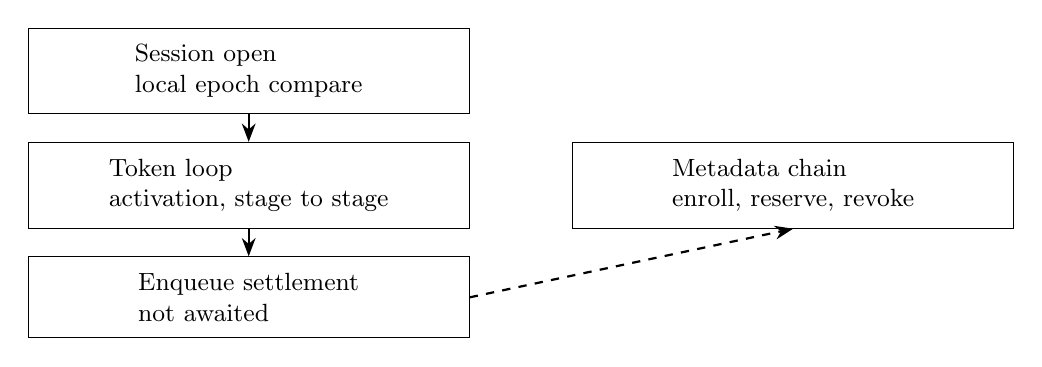
\begin{tikzpicture}[
  box/.style={draw, align=left, font=\small, inner sep=6pt, minimum width=5.6cm},
  arr/.style={-{Stealth}, thick}
]
\node[box] (a) {Session open\\local epoch compare};
\node[box, below=0.35cm of a] (b) {Token loop\\activation, stage to stage};
\node[box, below=0.35cm of b] (c) {Enqueue settlement\\not awaited};
\node[box, right=1.3cm of b] (d) {Metadata chain\\enroll, reserve, revoke};
\draw[arr] (a) -- (b);
\draw[arr] (b) -- (c);
\draw[arr, dashed] (c.east) -- (d.south);
\end{tikzpicture}
\caption{The token loop does not read or write the chain. Settlement is enqueued. A dashed edge is asynchronous.}
\label{fig:rails}
\end{figure}

\section{Evaluation methodology}
There is no device under test in this paper. The household measurements cited above were not repeated. The protocol that would be required before any public performance claim is: a named device, a frozen model file with a hash, a context length, cold and warm time to first token, a decode rate with the number of runs, energy if a battery claim is made, and a statement of what the coordinator captured. That protocol has not been run for community overflow.

What this paper does run is a deterministic calculator and a deterministic ledger.
\begin{itemize}
\item Admission uses the equations of Section~\ref{sec:admit} on the frozen geometry and on class floors. Class floors are not shipping SKUs, except the 128\,GB figure, which is the stated ThoxKey capacity.
\item Churn draws an independent Bernoulli leave for each contributor, seed 20261110, 200 trials. It does not model latency, partial stage failure, or bandwidth.
\item The grant drill walks the parent chain and the shred rule. It is not a penetration test and not an implementation of a production secrets service.
\item The ledger appends sixteen blocks and then attempts five illegal writes. Verification recomputes hashes.
\end{itemize}
Labels are CALCULATED for the arithmetic, SIMULATED for churn, grants, and the ledger, and MEASURED only for figures quoted from the household report.

\section{Calculated results}
\label{sec:results}
Table~\ref{tab:place} is the D23 planner at context 4096. The household floors are unplaceable under both D23 and the looser cross-check. Weight bytes exceed the 12\,GiB aggregate, so no rule that respects the file size will place the model there.

\begin{table}[t]
\centering
\small
\begin{tabular}{llc}
\toprule
Scenario & D23 & Cross-check \\
\midrule
2/4/6\,GB floors & unplaceable, 43 left & unplaceable, 34 left \\
one 16\,GB & unplaceable, 33 left & unplaceable, 23 left \\
one 32\,GB & unplaceable, 2 left & whole-request \\
one 64\,GB & whole-request & whole-request \\
two 16\,GB & unplaceable, 2 left & pipeline \\
two 32\,GB & pipeline & whole-request \\
three 16\,GB & pipeline, 0--30, 31--61, 62--63 & pipeline \\
pool with a 64\,GB host & whole-request on that host & whole-request \\
same pool, 64\,GB at P0 & pipeline on the 32\,GB hosts & whole-request \\
\bottomrule
\end{tabular}
\caption{Placement of frozen Qwen3.6-27B-Q4\_0 at context 4096. CALCULATED. The cross-check is not the code of record.}
\label{tab:place}
\end{table}

Seeded churn at leave probability 0.2 on the full pool placed 200 of 200 trials, 159 of them whole-request, because the 64\,GB host usually remained. Removing that host left 200 of 200 as pipelines and none as whole-request. Six 16\,GB hosts at leave probability 0.35 placed 182 of 200, all as three-stage pipelines, and left 18 unplaceable. These are simulations.

The product paths use the same planner. An idle 128\,GB key whole-requests every layer and spends 0 community credits. Held at owner priority, it is excluded, and three 16\,GB neighbors admit the pipeline at 3 credits. An 8\,GB class endpoint alone seats layers 0--14 and leaves 49. The same pipeline admits it. An idle hour of the key earns 76.8 credits and covers 25 such spills. A non-contributor grant of 8 credits covers 2 spills, with 2 credits left. None of these are prices.

The ledger fixture on that three-stage plan appends 16 blocks, verifies, and detects a one-field tamper of block 1 as a hash failure at index 1. The refused writes, none of which become blocks, are replay, double-spend, a credit transfer, a field named \texttt{prompt}, and a settlement after revoke. Payload bytes committed are 0. Subscriber endowment 8{,}000 milli-credits, reservation 3{,}000, remainder 5{,}000. The epoch advances from 1 to 2 on revoke. The grant drill accepts a matching principal, epoch, and fingerprint, and rejects a stale epoch, a cross-principal presentation, a mismatched fingerprint, and both descendants after the root is shredded.

For \(S=3\), \(H=2\), \(N=256\), and an assumed \(R=40\,\mathrm{ms}\), the rejected designs add 10.24\,s and 20.48\,s inside the token loop. The specification adds 0\,ms. Changing \(R\) changes only the rejected column.

\section{Security consequences}
The mesh inherits the household rule that the coordinator does not carry payloads, and adds a schema that rejects payload field names before a block is hashed. That is necessary and not sufficient. A stage process that unpickles an activation, or that accepts a peer before checking the grant, recreates CVE-2026-105192 on a different port. The required shape is typed records, a local allowlist of message kinds, peer authentication before decode, and no path on which a class name is taken from the message. This paper specifies that shape. It does not present a fuzzed implementation.

Timing side channels on the HMAC construction and on the epoch check are unexamined. Omission by the sequencer is detectable only by a subscriber who expected a block, not by hash verification of the chain that remains. There is no freedom-to-operate analysis in this document.

\section{Discussion}
Community overflow is justified where the household is honestly unplaceable and the subscriber would otherwise export the prompt. It is not justified as a faster path than a key that already holds the model. Whole-request has zero activation hops. A pipeline pays a hop per boundary on every token. Petals' own table shows that hop's round-trip time in the step rate. Adding a ledger commit to that hop would add another. The specification refuses the second addition and does not pretend the first is free.

The products stay in their roles. The key is the private whole-request runtime and, when idle, the largest credit earner in the pool. A small endpoint keeps the grant and does not pretend to hold the weights. Foreground work is priority P0 and is excluded. Credits account for memory-time. They are not a transferable instrument, which removes a class of market abuse and also removes any claim that this is a blockchain economy.

DICOMPUTE's caution applies directly. Distributed inference is most plausible for work that can be divided and that tolerates locality constraints. Tightly coupled, memory-intensive decode still prefers one host. Our planner encodes that preference by whole-request whenever one admitted node can hold the span.

\section{Limitations}
No device measurement, no wide-area trace, and no energy figure. The round-trip assumption is a pricing tool. Class floors are not bills of materials. The 128\,GB key is a stated product capacity, not a fresh measurement of usable bytes after the operating system. The sequencer is centralized. A partition can stall the audit log and must not stall decode, and a missing block must not be treated as permission to keep a dead epoch. Cross-principal KV reuse is unadmitted. Execution confidentiality is not claimed. The grant drill is a simulator.

\section{Context sweep, revision 0.4}
The reading copy of this specification is revision 0.4. The laboratory recomputes it. Two results are not in the 4096-only table above.

First, the three-host pipeline at context 4096 is tight. Each 16\,GB host has usable RAM $\lfloor 0.6 \times 16 \times 2^{30}\rfloor = 10{,}307{,}921{,}510$ bytes. The first stage, layers 0--30, requires $10{,}299{,}018{,}982$ bytes and clears admission by $8{,}902{,}528$ bytes. The second stage clears by one byte less. The third stage, layers 62--63, is the remainder, not a balanced share.

Second, KV grows with context and the reserve floor does not. At context 32768, D23 leaves 3 layers unplaced on one 64\,GB host while the printed cross-check still whole-requests it. Three 16\,GB hosts, a pipeline at 4096, leave 19 layers. Four 16\,GB hosts still leave 4. A sentence that says ``64\,GB holds the 27B'' is true at context 4096 under D23 and false at context 32768. The sweep is produced by \texttt{contextSweep} in the laboratory engine. Highlighted disagreements at 1024, 2048, 4096, and 8192 are the same three topologies: one 32\,GB host, two 16\,GB hosts, and two 32\,GB hosts.

\section{Conclusion}
The household already fails closed when a model does not fit, and it already keeps the coordinator off the payload. Community overflow is the admission of other principals' idle memory under a grant, with an audit log that cannot see the prompt and cannot sit on the token. The planner of record is stricter than the inequality printed in the household report, and the stricter rule is the one that decides whether a block may exist. The latency cost of that audit, inside the token loop, is zero by construction. Making that zero true on real links, on named devices, is future measurement. Until then the public claim is the architecture, the calculated placements, and the refusals.

\begin{thebibliography}{9}
\bibitem{mesh} C.~Ross and T.~Xaypanya, ``THOX MeshStack: Capacity-Priced Pipeline Sharding, Grant-Gated KV Transfer and Lease-Fenced Device Roles for a Private Household Mesh,'' THOX.ai Research technical report v1.1.0, 2026. Concept DOI 10.5281/zenodo.23919579. Repository citation records version DOI 10.5281/zenodo.23969070. Public HTML edition states the version DOI as pending.
\bibitem{petals} A.~Borzunov, D.~Baranchuk, T.~Dettmers, M.~Ryabinin, Y.~Belkada, A.~Chumachenko, P.~Samygin, and C.~Raffel, ``Petals: Collaborative Inference and Fine-tuning of Large Models,'' in \emph{Proc.\ ACL}, System Demonstrations, pp.~558--568, 2023. DOI 10.18653/v1/2023.acl-demo.54. arXiv:2209.01188.
\bibitem{lmcache} Y.~Liu, Y.~Cheng, J.~Yao, Y.~An, X.~Chen, S.~Feng, Y.~Huang, S.~Shen, R.~Zhang, K.~Du, and J.~Jiang, ``LMCache: An Efficient KV Cache Layer for Enterprise-Scale LLM Inference,'' arXiv:2510.09665, submitted 8~October 2025. Abstract reports up to 15$\times$ throughput with vLLM. External datacenter result. No latency multiplier is imported from this paper.
\bibitem{cacheblend} J.~Yao et~al., ``CacheBlend: Fast Large Language Model Serving for RAG with Cached Knowledge Fusion,'' arXiv:2405.16444, 2025. External serving-stack result.
\bibitem{dicompute} R.~Kakkad, A.~Khekade, A.~Chinchawale, O.~Mestry, and B.~Mohammadkhani, ``DICOMPUTE: An Economic and Privacy-Aware Framework for Distributed Artificial Intelligence Inference,'' arXiv:2611.10804, 2026.
\bibitem{ct} B.~Laurie, A.~Langley, and E.~Kasper, ``Certificate Transparency,'' RFC~6962, 2013.
\bibitem{cve} JFrog Security Research (Yuval Moravchick), ``LMCache unauthenticated remote code execution via pickle deserialization on the multiprocess ZeroMQ transport,'' CVE-2026-105192, disclosed 7~October 2026. CVSS 3.1 base 9.8. Fixed in LMCache 0.5.6 (14~October 2026) by typed MessagePack descriptors and a local allowlist. Default bind is localhost.
\end{thebibliography}

\section*{Reproducibility}
Admission, the cross-check, churn, the grant drill, and the ledger are produced by \texttt{src/lib/lab/engine.mjs} and \texttt{src/lib/lab/ledger.mjs} in the laboratory that accompanies this specification. Geometry fingerprint \texttt{b4302c31c5d0b72435044638ad961409d7d4feeb354d3dadad4fd2777bf955e6}. Churn seed 20261110. No new measurement files are released. arXiv packaging: this file, pdflatex, no external links required to compile. An arXiv identifier does not yet exist, so Hugging Face paper indexing is not available.

\section*{Generative AI assistance disclosure}
Synthetic agents assisted with literature search, repository review, and drafting. They are not authors. Technical claims, evidence labels, the decision to keep D23 when it disagrees with the printed household inequality, and the decision to keep the ledger off the token path were reviewed by the human authors and remain their responsibility.
\end{document}
